\documentclass[12pt]{article}
\usepackage{html}
\usepackage{graphicx}
\usepackage{palatino}
\usepackage{setspace}
\usepackage{amsmath}
\usepackage{boxedminipage}
\usepackage{colortbl}
\usepackage{color}
\usepackage{chicago}
\onehalfspacing


\newcommand{\bgamma}{\mbox{\boldmath $\Gamma$}}
\newcommand{\bL}{\mbox{\boldmath $L$}}
\newcommand{\bT}{\mbox{\boldmath $T$}}
\newcommand{\bI}{\mbox{\boldmath $I$}}
\newcommand{\bM}{\mbox{\boldmath $M$}}
\newcommand{\bm}{\mbox{\boldmath $m$}}
\newcommand{\bN}{\mbox{\boldmath $N$}}
\newcommand{\bE}{\mbox{\boldmath $E$}}
\newcommand{\bA}{\mbox{\boldmath $A$}}
\newcommand{\bB}{\mbox{\boldmath $B$}}
\newcommand{\bK}{\mbox{\boldmath $K$}}
\newcommand{\bP}{\mbox{\boldmath $P$}}
\newcommand{\bx}{\mbox{\boldmath $x$}}
\newcommand{\bU}{\mbox{\boldmath $U$}}
\newcommand{\bV}{\mbox{\boldmath $V$}}
\newcommand{\bZero}{\mbox{\boldmath $0$}}
\newcommand{\bLo}{\mbox{\boldmath $L_0$}}
\newcommand{\bNo}{\mbox{\boldmath $N_0$}}
\newcommand{\bNr}{\mbox{\boldmath $N_R$}}
\newcommand{\bSi}{\mbox{\boldmath $S_i$}}
\newcommand{\bSd}{\mbox{\boldmath $S_d$}}
\newcommand{\bdSi}{\mbox{\boldmath $dS_i$}}
\newcommand{\bdSd}{\mbox{\boldmath $dS_d$}}
\newcommand{\bS}{\mbox{\boldmath $S$}}
\newcommand{\bdS}{\mbox{\boldmath $dS$}}
\newcommand{\bdt}{\mbox{\boldmath $dt$}}
\newcommand{\bdSdt}{\mbox{$\displaystyle \frac{\bdS}{\bdt}$}}
\newcommand{\bdSddt}{\mbox{$\displaystyle \frac{\bdS_d}{\bdt}$}}
\newcommand{\bdSidt}{\mbox{$\displaystyle \frac{\bdS_i}{\bdt}$}}
\newcommand{\bv}{\mbox{\boldmath $v$}}
\newcommand{\bp}{\mbox{\boldmath $p$}}

\parindent=0pt
\parskip=4pt

\begin{document}
\thispagestyle{empty}

\onecolumn

\title{Standards, Platforms \& Applications}

\author{\thanks{Address for Correspondence: Herbert
M Sauro, Keck Graduate Institute, 535 Watson Drive, Claremont,
USA, 91711 Phone: (909) 607 0377  Fax: (909) 607 8086 e-mail:
hsauro@kgi.edu, web page www.sys-bio.org} Herbert M.\ Sauro, \\
Keck Graduate Institute, \\ 535 Watson Drive, Claremont, USA,
91711 \\ }

\maketitle
\vspace{3in} Running Title: Standards, Platforms \& Applications
 \clearpage

\pagebreak

\section*{Summary}

With the sequencing of the human genome, it has become apparent that Systems Biology, the understanding of cellular networks through dynamical analysis is becoming an important
part of research for mainstream biologists. One of the indicative trends to emerge in recent years is the development of model interchange standards that permit biologists to easily exchange dynamical models between different software tools. In this chapter
two chief model exchange standards, SBML and CellML are described. In addition,
the development of extensible software frameworks, including SBW, BioSPICE and
BioUML are discussed and the role they might play in stimulating the development
of new tools and approaches. Finally, the range of possible computational applications is
described, highlighting the rich set of tools that is emerging as systems biology
becomes a mainstream science.

\pagebreak

\section{Introduction}

Although Computational Systems Biology may seem to be a recent
field of endeavor, its origins can be traced as far back as the
1920s and 30s \cite{Wright1929}. During this period it was already
believed by some that genes were responsible in some way for
specifying enzymes. It was also around this time that glycolysis,
the first metabolic pathway, was being elucidated and the
beginnings of the idea that enzymes formed linked sequences called
pathways. It is even more remarkable therefore that given the
infancy of these concepts, Sewell Wright should attempt to give a
physiological explanation for the occurrence of genetic dominance
and recessivity \cite{Wright1934}. Wright argued that the
explanation for the origin of dominance lay with the properties of
catalytic networks, and laid out an initial mathematical theory
which described the properties of enzyme networks\footnote{This
early work later became significant during the development of
metabolic control analysis \cite{KB81}}. In the 1940's, as the
first digital computers were being built, pioneering individuals such as 
Garfinkel, Higgins and Chance began investigating the possibility of 
modelling the subtle behavior of biochemical pathways. Even before the
advent of the digital computer, the same group had been using using 
analog computers to model simple biochemical pathways for almost 15 years \cite{Ga61,Hi59,Chance1943}.

Since the work of the pioneers in the 1950's, there have been many
small groups that have continued this line of inquiry and that
together laid the foundation for many of the techniques and
theory that we use today and take for granted, in contemporary
systems biology. It should be noted that there is a large body of
literature, particularly in the Journal of Theoretical Biology,
dating back fifty years that many newcomers to the field will find
useful to consider.

\subsection{What is Systems Biology?}

There are many conflicting opinions today on what exactly systems
biology is. Historically the answer seems clear. The chief aim of
systems biology is to understand how individual proteins,
metabolites and genes contribute quantitatively to the phenotypic
response. Lee Hood, president of the Institute of Systems Biology
in Seattle, US, defines it similarly as "the identification of the
elements in a system and the analysis of their interrelationships
so as to explain the emergent properties of the system". Even so,
some believe systems biology to be concerned with the collection
of high-throughput data while others consider the elucidation of
protein-protein networks and gene networks to be its hallmark.
Certainly, both are vital prerequisites for understanding systems
but neither alone can offer great {\em insight} into how networks
operate dynamically.

Systems Biology is the natural progression of classical molecular
biology from a descriptive to a quantitative science and is
concerned with the dynamic response of biological networks.

\subsection{Statement Of Problem}

Building models is not an entirely new approach to biology. If one
examines any text book on molecular biology or biochemistry,
virtually every page has a diagram of a model. These models,
which are often termed cartoon based models, represent the culmination
of years of painstaking research; they serve as repositories of
accepted doctrine and the starting point for the generation of new
hypotheses. There are, however, limits to what can be done with
these models, their predictive value tends to be poor, and
the ability to reason using qualitative models is limited. In
other sciences these limitations are avoided through the use of
quantitative models, models which are described not just
pictorially but also mathematically. Quantitative models by their
nature have much better predictive value compared to qualitative
models, but their real usefulness stems from the capacity to carry
out precise reasoning with them.

\section{Quantitative Approaches}

There is a wide range of mathematical representations that one can
use to build quantitative models, the choice of approach depending
on the type of biological question, the accessibility of
experimental data and the tractability of the mathematics. A short
list of modelling representations is given in Figure 1. Probably the most successful and
widely used kind of model are those based on differential
equations (both ordinary and partial). These models assume a
continuum of concentrations and rates. In reality of course,
cellular systems are discrete at the molecular level, however,
since the numbers of molecules is very large, the continuum
approximation turns out to be very good. When the number of
molecules drops to below a certain threshold the continuum model
can break down and in these cases one must revert to stochastic
simulation. The disadvantage of a stochastic simulation is that
all the analytical methods available for continuous models no
longer apply. One should therefore only use stochastic simulation
if it is absolutely necessary and not in cases where an ODE based
model adequately describes the data. This problem highlights the need to develop a
new set of mathematical approaches in order to understand the dynamics of
stochastic systems. There are other approaches, which
include boolean, bayesian, formal logic and connectivity studies
but these have yet to show any overwhelming advantage over
continuum based models.

In this chapter I will be exclusively concerned with models based
on differential equations and to a lesser extent stochastic
equations.

\begin{figure} \label{table:mathTechniques}
\rule[-5pt]{14cm}{1pt}
\begin{description} 
\item[Boolean:] One of the simplest possible modelling techniques
is to represent a network using Boolean logic \cite{DeJong2002}.
This approach has been used to model gene networks.
%
\item[Ordinary differential equations (ODEs):] This is the
commonest and arguably most useful representation. Although based on
a continuum model, ODE models have proved to be excellent descriptions
of many biological systems. Another advantage to
using ODEs is the wide range of analytical and numerical methods that are available. The
analytical methods in particular provide a means to gain a deeper
insight into the workings of the model.
%
\item[Deterministic hybrid:] A deterministic hybrid model is one
which combines a continuous model (e.g ODE model) with discrete
events. These models are notoriously difficult to solve efficiently and
require carefully crafted numerical solvers. The events can occur
either in the state variables or parameters and can be
time dependent or independent. A simple example involves the
division of a cell into two daughter cells. This event can be
treated as a discrete event which occurs when the volume of the
cell reaches some preset value at which point the volume halves.
%
\item[Differential-algebraic equations (DAEs):] Sometimes a model
requires constraints on the variables during the solution of the
ODEs. Such a situation is often termed a DAE system. The simplest
constraints are mass conservation constraints, however these are
linear and can be handled efficiently and easily using simple
assignment equations (see equation \ref{eq:general}). DAE solvers need only
 be used when the constraints are nonlinear.
%
\item[Partial differential equations (PDEs):] Whereas simple ODEs
model well stirred reactors, PDEs can be used model heterogenous
spatial models. 
%
\item[Stochastic:] At the molecular level concentrations are
discrete, but as long as the concentrations levels are sufficiently high,
the continuous model is perfectly adequate. When concentrations
fall below approximately one hundred molecules in the volume considered (e.g. the cell or compartment) has to consider using stochastic modelling. The great disadvantage in
this approach is that one looses almost all the analytical methods
that are available for continuous models, as a result stochastic
models are much more difficult to interpret. 
\end{description}
\rule[6pt]{14cm}{1pt}
\caption{ A non-exhaustive selection of mathematical techniques for modelling biological systems.}
\end{figure}


\subsubsection{Quantitative Models Based on Differential Equations}

It is probably fair to say that most of the successful models to
be found in the literature are based on ordinary differential
equations. Many researchers will express these models using the
following equation:

\begin{equation}
\frac{\bdS}{\bdt} = \bN \bv (\bS (\bp), \bp) \label{eq:system}
\end{equation}

where $\bS$ is the vector of molecular species concentrations,
$\bN$, the stoichiometry matrix; $\bv$ the rate vector and $\bp$ a
vector of parameters which can influence the evolution of the
system. Real cellular networks have an additional property that is
particularly characteristic of biological networks, this is the
presence of so-called moiety conserved cycles. Depending on the
time-scale of a study, there will be molecular subgroups conserved
during the evolution of a network, these are termed {\em conserved
moieties} \cite{Re81}. The total amount of a particular moiety in
a network is time invariant and is determined solely by the
initial conditions imposed on the system\footnote {There are rare
cases when a `conservation' relationship arises out of a
non-moiety cycle. This does not affect the mathematics but only
the physical interpretation of the relationship. For example, A
$\rightarrow$ B + C; B + C $\rightarrow$ D has the conservation,
$B - C =\mbox{constant}$, }.

In metabolism, conserved cycles act as common conveyers of energy (ATP) or reducing power (NAD); in signaling pathways they occur as protein phosphorylation states while in genetic networks, they occur as bound and unbound protein states to DNA. These conserved cycles will often have a profound effect on the network behavior and it is important that they be properly considered in computational models.

From the full set of molecular species in a model, it is customary
to divide the set into two groups, the dependent ($\bSd$) and
independent set ($\bSi$). This division is dependent entirely on
the number and kind of conserved cycles in the network. If there aren't any conserved
cycles in a model then the dependent set is empty and the size of
the independent set equals the number of molecular species in the
model. For details on how to compute $\bSd$ and $\bSi$ the reader
should consult \cite{Sauro:ICycles2004}.

Equation (\ref{eq:system}) is therefore better expressed as:

{ \addtolength{\jot}{6pt}
\begin{eqnarray}
  \bSd &=& \bLo \bSi + \bT \nonumber \\
  \bdSidt &=& \bNr \bv (\bSi (p), \bSd, \bp) \label{eq:general}
\end{eqnarray} }

In these equations, $\bSi$ is the vector of independent species,
$\bSd$, the vector of dependent species, $\bLo$ the link matrix,
$\bT$ the total mass vector, $\bNr$ the reduced stoichiometry
matrix, $\bv$ the rate vector and $\bp$ the vector of parameters. Equation (2)
constitutes the most general expression of an ODE based temporal model \cite{hofmeyr-nutshell,Schuster:Book}. The symbolism used in equation (2) is the standard
notation used by many in the Systems Biology community. 

Although mathematically, reaction based models are given by
equations (\ref{eq:system}) and (\ref{eq:general}), many researchers
are more familiar with expressing models in the form of a reaction scheme. For example, 
the following describes part of glycolysis:

\begin{figure}[h]  \label{figure:script}
{\small
\begin{verbatim}
  Glucose-6-P -> Fructose-6-Phosphate
  Fructose-6-Phosphate + ATP -> Fructose-1-6-Bisphosphate + ADP
  Fructose-1-6-Bisphosphate -> DHAP + GAP
\end{verbatim} }
\caption {Part of Glycolysis described using a reaction scheme notation.} 
\end{figure}


For brevity, the rates laws that accompany each
reaction have been left out. Such notation is well understood by biologists.
It is not straight forward however  to convert this representation to the
representation give by equation (\ref{eq:general}). However, many software
tools will permit users to enter models as a list of reactions and
then automatically generate the mathematical model
\cite{SauroF91,sauro:2000,Sauro:Omics}.

\medskip

\setlength\fboxsep{18pt}
\begin{boxedminipage}[hbp]{14cm}
{\bfseries Box 1. Reaction Network} Consider the simple reaction
network shown on the left below:

\begin{minipage}[t]{6cm}
\begin{picture}(60,95)(-60,-50)\thicklines
%
\put(18,20){$v_2$}
\qbezier(0,0)(20,20),(40,0) \put(42,-1){\vector(4,-3){2}}
%
\put(16,-46){$v_3$}
\qbezier(0,-20)(20,-40),(40,-20) \put(0,-19){\vector(-3,4){2}}
%
\put(-9,-12){$ES$}
\put(40,-13){$E$}
\put(65,23){$S_1$}
\put(65,-48){$S_2$}
\put(69,16){\vector(0,-1){48}}
\put(72,-8){$v_1$}
%
% Lower arm
\qbezier(62,-45)(20,-40),(0,-20)
% Upper arm
\qbezier(18,10)(26,8),(60,25) \put(61,25){\vector(2,1){2}}
%
\end{picture}
\end{minipage}
\begin{minipage}[t]{6cm}
\begin{picture}(60,85)(-40,-35)\thicklines
  % Vertical arrows
  \put(-9, 24){$ES$}
  \put(-9, 8){$S_1$}
  \put(-9, -11){$S_2$}
  \put(-9, -26){$E$}

  \put(26,40){$v_1$}
  \put(46,40){$v_2$}
  \put(68,40){$v_3$}

$\begin{array}{cc}
        \left[
         \begin{array}{rrr}
            0 & -1 &  1  \\
           -1 &  1 &  0  \\
            1 &  0 & -1  \\
            0 &  1 & -1
         \end{array}
        \right]
   \end{array}$
\end{picture}
\end{minipage}

\vspace{12pt} The {\bfseries stoichiometry matrix} for this
network is shown to the right. This network possesses two
conserved cycles given by the constraints: $S_1 + S_2 + ES = T_1$
and $E + ES = T_2$. The set of independent species includes:
$\{ES, S_1\}$ and the set of dependent species $\{E, S_2 \}$.

\bigskip
The $\bLo$ matrix can be shown to be:

\hspace{2cm} $$ \bLo = \left[ \begin{array}{rr}
  -1 & -1 \\
  -1 & 0 \\
\end{array}  \right]$$ \hfill
%
\linebreak
The complete set of equations for this model is therefore:

$$
\left[ \begin{array}{l}
  S_2 \\
  E \\
\end{array} \right] =
\left[ \begin{array}{rr}
  -1 & -1 \\
  -1 & 0 \\
\end{array}  \right]
\left[
\begin{array}{l}
    ES \\
    S_1 \\
\end{array}
\right] +
\left[
\begin{array}{l}
  T_1 \\
  T_2 \\
\end{array}
\right]$$
$$\left[
\begin{array}{l}
  dES/dt \\
  dS_1/dt \\
\end{array}
\right] =
\left[
\begin{array}{rrr}
  0 & -1 & 1 \\
  -1 & 1 & 0 \\
\end{array}
\right]
\left[
\begin{array}{l}
  v_1 \\
  v_2 \\
  v_3 \\
\end{array}
\right]$$ Note that even though there appears to be four variables
in this system, there are in fact only two independent variables, $\{ES, S_1\}$,
and hence only two differential equations and two linear constraints.

\end{boxedminipage}

%\pagebreak

\section{Standards}

In recent years, particulary since the sequencing of the human
genome, there has been an ever increasing list of wide ranging
cellular models published in the literature. Each author has a
particular notation that they use to publish the model. Some authors
will publish the model as a reaction scheme, much like the
notation given in Figure 2. Others will itemize the actual
mathematical representation in the form of a list of differential
equations. Some authors do not publish the model at all but
provide the model as supplementary information. Until recently,
there has been no way to publish models in a standard format.
Without a standard format it has proved very difficult if not
impossible in many cases to use published models without
considerable effort.

As a result of this obvious shortcoming, a number of groups set
out to gather community support to develop a standard that model
developers would be happy to use.  There was an early effort in
1998 by the BTK (BioThermoKinetics) group to standardize on a
practical format for exchanging models between Gepasi
\cite{Gepasi:1993} and SCAMP \cite{SauroF91}, both tools were
widely used at the time. Around the same time, bioengineers at the
University of Auckland began investigating the role that XML \cite{harold:2001} could
play in defining a standard for exchanging computational models in
order to reduce errors that appeared frequently in published
models. From the Auckland team emerged CellML
\cite{LloydCellML2004}. Members from the BTK group subsequently
took their experience and contributed significantly to the other
major model exchange standard, called SBML \cite{hucka:2002d}.
SBML was developed in 2000 at Caltech, Pasadena as a result of
funding received from the Japanese ERATO program. Both CellML and
SBML are today viewed as the main standards for exchanging
cellular network models. There are however fundamental differences
between the approaches that CellML and SBML take in the way models
are represented.


\subsection{CellML}

CellML \cite{LloydCellML2004} represents cellular models using a
mathematical description similar to equation (\ref{eq:system}). In
addition, CellML represents entities using a component based
approach where relationships between components are represented by
connections. In many ways CellML represents a literal translation
of the mathematical equations, except that the relationship
between dependent and independent species is implied rather then
explicit. The literal translation of the mathematics however goes
much further, in fact the representation that CellML uses is very
reminiscent of the way an engineer might wire up an analog
computer to solve the equations (though without specifying the integrators). As a result CellML is very general and in principal could probably represent any system that
has a mathematical description (and not just the kind indicated by equation (1)). CellML is also very precise in that every item in a model is defined explicitly. However, the
generality and explicit nature of CellML also results in
increased complexity especially for software developers. Another
side effect of the increased complexity is that models that are
represented using CellML tend to be quite large. On average, my
own analysis of a sample from the CellML repository \url{www.cellml.org/examples/repository/}
indicates that each reaction in a model requires about 5Kbytes of
storage.

Another key aspect of CellML is its provision for metadata
support. The metadata can be used to provide a context for a
model, such as the author name, when it was created and what
additional documents are available for it's description. CellML
uses standard XML based metadata containers such as RDF and within
RDF the Dublin Core.

The CellML team has amassed a very large suite (hundreds) of
models which provides many real examples of CellML syntax. This is
an extremely useful resource for the community.

Owing to the complexity of CellML, one unfortunate side effect
is that there are very few tools which can read and write CellML.
As far as the author is aware there are only two third-party tools
that can read and write CellML, these are VCell \cite{VCELL} and COR \cite{COR2003}. The
CellML team have recently (2004, http://cellml.sourceforge.net/)
began to provide their own software tools to third-party
developers. The delay in providing such tools to the community is
probably one reason why CellML (given it's complexity) has not
proved so popular relative to SBML which I will discuss next.


%For example, consider
%the system:
%
%\begin{center}
%$ A \xrightarrow{v_1} B \xrightarrow{v_2} C $
%\end{center}
%
%where A, B and C are molecular species and the arrows represent
%chemical transformations with rates $v_1$ and $v_2$. CellML
%effectively represents this both in the following way:

\subsection{SBML}

Whereas CellML attempts to be highly comprehensive, SBML was
designed to meet the immediate needs of the modelling community and
is therefore more focused on a particular problem set. One result of
this is that the standard is much simpler and much less verbose.
Like CellML, SBML is based on XML, however unlike CellML, it takes
a different approach to representing cellular models. The way
SBML represents models closely maps the way existing modelling
packages represent models. Whereas CellML represents models as a
mathematical wiring diagram, SBML represent models as a list of
chemical transformations much like the example indicated in Figure 2. Since every process in a biological cells can ultimately be broken down into one or more chemical
transformations this was the natural representation to use.
However SBML does not have generalized elements such as
components and connections, SBML employs specific elements to
represent spatial compartments, molecular species and chemical
transformations. In addition to these, SBML also has provision for
rules which can be used to represent constraints, derived values
and general math which for one reason or another cannot be
transformed into a chemical scheme. Like CellML, the dependent and
independent species are implied.

\subsubsection{SBML Development Tools}

Early on in the development of SBML, the original authors decided
to provide software tools almost immediately for the community.
Since XML at the time was not well understood by many software
developers the provision of such assistance was crucial. In
hindsight, this is probably one reason why SBML has become
a popular standard. Initially the original authors provided a simple
library for the Windows platform since the bulk of biology based
users tend to be Windows users. Today this library is still used
by a number of tools including Gepasi, Jarnac and JDesigner. With
the growing popularity of SBML, the community has since developed
a comprehensive cross platform tool (\url{http://sbml.sourceforge.org}) which is now
the recommended SBML toolkit to use (libSBML). libSBML was developed in C/C++ for maximum
portability.

\subsubsection{Extensibility}

It was realized early on by the authors of SBML that as systems
biology developed there would be pressure from the community to
make additional functionality available in SBML. To address this
issue, SBML has a formal means for adding extensions in the form
of the so-called annotations. There now exist a number of annotations
that are used by software developers. Some of these address issues
such as providing visualization information to allow software
tools to render the model in some meaningful way (two examples of
these will be given in a later section). Other extensions provide
a means to store information necessary for flux balance analysis
or to provide information for stochastic simulations. Ultimately
some of the extensions will most likely be folded into the
official SBML standard. This mechanism, a sort of Darwinian
evolution, permits the most important and popular requests to be
made part of SBML. It makes the process of SBML evolution more
transparent and permits users to be more involved in the
development of SBML.

\subsubsection{Practical Considerations}

While CellML is very general, SBML is more specific, as result,
the storage requirement for SBML is much less. It takes on average
roughly 1.5Kbytes to store a single chemical transformation in SBML
Level 2 (compared to 5K for CellML). Interestingly it only takes
roughly 50 to 100 bytes to store single transformations in raw
binary format where there is minimal extraneous syntax. Some
readers may feel that with today's cheap storage technologies,
that discussions on storage requirements is unnecessary. Indeed
for small models it is not an issue. However, in future very large
models are likely to be developed. There is, for example a serious
attempt (www.physiome.org) now underway to model in the
long term entire organs and even whole organisms. The amount of
information in these cases is huge and the question of efficient
storage is not so trivial. Obviously XML is highly compressible
and large models can be stored in this way. However, inefficient
storage also increases the time taken to manipulate the models.
Furthermore, in a modelling environment, model authors tend to
generate hundreds of variants while developing the model. For a
large model this clearly would generate huge amounts of XML based
data. One of the things that has yet to be addressed by either
standard is the how model variants can be efficiently stored.

\subsubsection{Usage}

Both SBML and CellML have been taken up by many software developers and implemented in their software. SBML in particular is being used in over 75 software projects. In addition, SBML is the official model interchange format for the BioSPICE project \url{www.biospice.org}, the SBW project \url{www.sys-bio.org}, the international {\em E.\ coli} alliance and the receptor tyrosine kinase consortium. Much of the SBML support is in stand-alone applications, however, a number of database vendors have also decided to provide export of SBML as an option, examples include reactome, stke and sigpath.

A related standard that has been proposed by \cite{MFAML2004} is
for the storage of flux balance models. The proposed format is
very similar to SBML but has the additional feature of storing the
flux balance objective function.

\subsection{Future Considerations}

The development of standards for systems biology is still at a
very early stage. I have not for example considered the problem of
standardizing the formats for the experimental data that will be
required for modelling. For example, there are no current standards
for representing {\em quantitative} proteomic or metabolomic data, though efforts
for defining a quantitative microarray format is maturing (\url{www.mged.org).

More pressing from a modelling perspective is that there is currently no agreed way to merge smaller sub-models into larger models (composition). One of the few groups to have considered composition is Ginkel and Kremling \cite{Promot2000}. They have examined possible extensions to SBML to allow SBML to represent sub-models and models composed of sub-models. Additional issues include distinguishing different kinds of models, particularly ODE and stochastic models, currently there is no means to identify the kind of model an SBML file represents other than to use specific annotations. One unfortunate side-effect of using XML is the temptation to omit a detailed semantic specification. XML is often vaunted as a desirable technology because it is easily parsed, however, parsing and syntax checking is a very easy task to implement, the real difficulty comes when semantic checks are required and current XML technology offer no assistance in this task.

\subsection{Other Standards}

Apart from using XML to define an interchange format, there are two other mediums
for representing models, these include, human readable text based formats and
visual formats.

\subsubsection{Visualization of Models}

For many users, the ability to visualize models and to build
models using visual tools is an important feature. There are currently
a number of visualization formats that are in common use. One of the
most comprehensive and freely available formats is the molecular interaction
maps developed by Kohn \cite{Kohn1999} and more recently by Mirit Aladjem \cite{Kohn2004}. The
Kohn format emerged from the need to represent complex signaling networks in
a compact way. Unlike metabolic networks, signalling networks can be extremely
complex with multiple protein states and interactions and therefore an alternative and more
concise approach is desirable. At the time of writing
there is no software for manipulating Kohn maps and no means to convert
Kohn maps to SBML or any other standard. Hopefully this will change in the future.

An early computer based visual notation was proposed by Cook \cite{Cook2001} who developed
a notation called BioD. This notation has been implemented in a commercial software package
called KineCyte \linebreak (http://www.rainbio.com/Software.html).

Another proposal has been put forward by Kitano \cite{Kitano2003}. This is a more traditional
approach where different molecular entities (such as proteins, ions, transporters etc.) have particular pictorial representations. The software tool called cellDesigner \cite{CellDesigner2003} implements this proposed format.

One of the first visualization tools, JDesigner \cite{Sauro:Omics} also implements a
traditional way to depict networks (see Figure 3) using a pictorial representation to indicate substances and reactions. JDesigner also employs bezier curves to represent arcs in an attempt to make the diagrams similar to the notation found
in many molecular biology text books. CellDesigner and JDesigner connect to the Systems Biology Workbench (SBW) for simulation support.

\begin{figure}[h] \label{Figure:JDesigner}
\begin{center}
  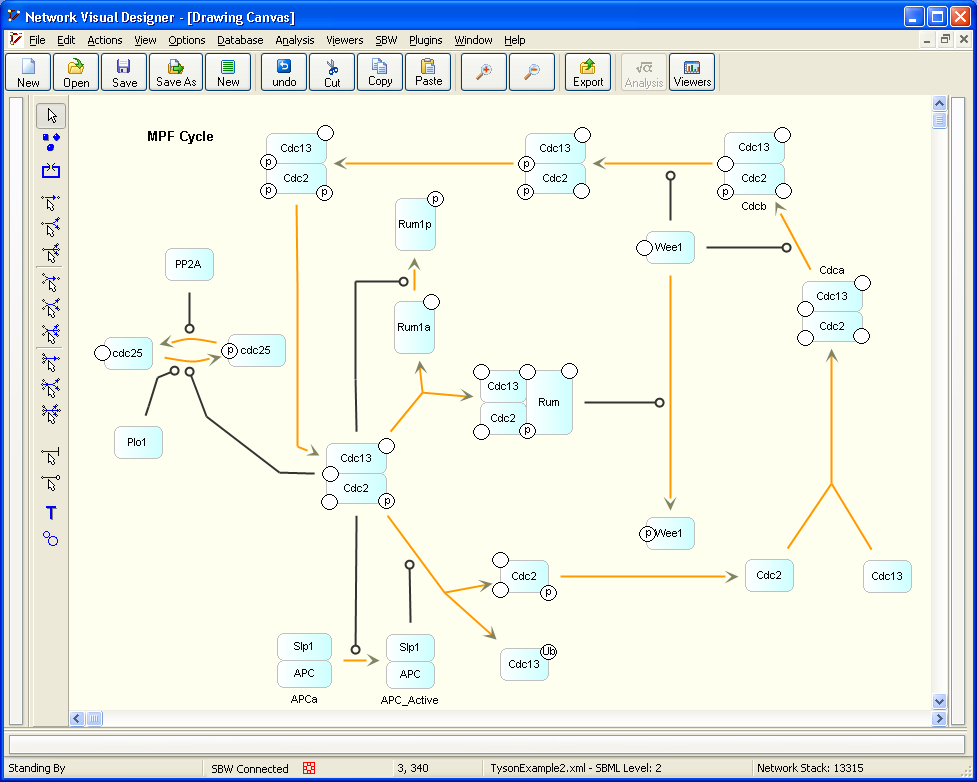
\includegraphics[width=4.5in,height=4in]{JDesigner1.eps}
\end{center}
\caption{Example of JDesigner's visual format}
\end{figure}


Finally, there is a proposal from a commercial company called Gene Network Sciences which has
devised a derivative of the Kohn notation called DCL. However this notation is proprietary and it's utility to the general scientific community is not certain at this time.

\subsubsection{Human Readable Formats}

In addition to visualization approaches and the use of XML to represent models, there has been a long tradition in the field to describe models using human readable text based formats. Indeed the very first simulator BIOSSIM, \cite{Ga68}, allowed a user to describe a model using a list of reaction schemes. Variants of this have been employed by a number of simulators since, including, SCAMP \cite{SauroF91}, Jarnac \cite{sauro:2000}, E-Cell \cite{ECELL} and more recently Pysces \cite{Pysces2005}. Being able to represent models in a human readable format offers many advantages, including, conciseness, easily understood and manipulated using a simple editor, flexible, portable and above all extremely easy to include commenting and annotation.

\subsection {Model Databases}

At the time of writing there are, surprisingly, no model databases
currently in existence. There are databases for almost every other
kind of biological information except dynamic information. This is even
more surprising since dynamic behavior is probably {\em the} key feature
of biological systems. 

There are a number of sites which include simple lists of models, for example the CellML Repository, but there are no searchable databases. Although such databases would
be of great advantage to the community, the funding agencies have
so far been reluctant to provide support. Instead a number of
groups, including the original SBML group and the SBW group are
instead developing model databases as part of other projects. In
particular the Department of Energy through their GTL program are
funding a small project to develop a database for microbial
models. What features of a database might be useful? Probably one
of the most useful features for such a database (apart from the
obvious ability to query the database for particular models, organisms etc)
would be the ability to deliver models in different computationally ready formats.

\subsection{Other Related Standards}

CellML and SBML are the primary formats used to store interchangeable dynamic models. Apart from the particular details on the model itself there is also the need to consider data that is used to build the models. Most models are built by laboriously searching the literature and carrying out additional experiments as necessary to fill in gaps in the data. This has proved to be an extremely effective method to building reliable models \cite{TysonNatReview2001,TysonBioessay2002}. However, Many inexperienced researches in Systems Biology feel that high-throughput data is the answer to the needs of the modelling community. Unfortunately much of the high-throughput data that is currently available is not appropriate. Much of the high-throughput data is very noisy and is probably more suitable for building qualitative models. More importantly, the bulk of high-throughput data is not generated with dynamic model building in mind and therefore is often not appropriate for this purpose. To date there has not been a single dynamic model that has been constructed as a result of high-throughput data. As systems biology and the construction of dynamic models becomes more important, it is very likely that the utility of high-throughput data will become much more significant. When this happens a proposed standard, called BioPAX (www.biopax.org) will most likely contribute.

BioPAX (Biological Pathway Exchange) is another proposed standard
based on XML. BioPAX aims to integrate many of the incompatible
pathway related databases (such as BioCYC, BIND, WIT, aMAZE, KEGG
and others) so that data from any one of these databases can be easily
interchanged. In future it should be possible to extract data from
many of the pathway databases and integrate the data directly into
SBML (or CellML) via BioPAX. The BioPAX group proposes to embed BioPAX 
elements onto SBML or cellML for unambiguous identification of 
substances (metabolites, enzymes) and reactions.


\section{Platforms}

Much of the current software development in the systems biology
community concentrates on the development of stand-alone
applications. Most of these tools are not easily extensible and
many of them offer nearly identical functionality. One of the
problems that currently plagues systems biology is the continual
reinvention of the same kind of tool (called YADS - yet another
differential equation solver). I believe it is not too unfair to
suggest that in many cases our software capability today in
systems biology is only marginally better than the first systems
biology simulation package ever written (BIOSSIM) by David
Garfinkel around 1960 \cite{Ga68}. In many cases even the user
interfaces are only marginally better. There are of course
exceptions to this, VCell \cite{VCELL} in particular comes to mind as
well as tools such as Gepasi \cite{Gepasi:1993} and Jarnac/JDesigner \cite{Sauro:Omics}.
VCell is particularly suited to spatial modelling, Gepasi is well known for it's
GUI user interface, the selection of optimization methods and it's ability to fit data to models, Jarnac was until very recently (See Pysces \cite{Pysces2005}) the only script based programmable modelling tool which has a fairly complete set of tools for the analysis of time dependent ODEs and stochastic systems and finally JDesigner because it was the first visual design model tool.

The reason for the repetitive nature of software in systems biology is that almost each and every group engaged in computational systems biology writes their own simulation package. Given the time constraints on the project, the software will only reach a level
of maturity that is often equivalent to BIOSSIM. As a result, the
provision of software does not appear to advance.

A number of groups have recognized this problem and instead of
developing single isolated applications, they have chosen to
develop a software infrastructure that permits and encourages
extensibility and code reuse. The later is extremely important as
it allows developers to build on existing code which in turn leads
to new and interesting software tools. In this section I will
describe three such environments, SBW, BioSPICE and BioUML. All three
environments are open source.


\subsection{SBW - Systems Biology Workbench}

The SBW (Sauro et. al., 2004) is an extensible software framework
that is both platform and language independent. Its primary
purpose is to encourage code reuse among members of the systems
biology community. Developers can run SBW on Linux, Windows or Mac
OS and can develop software in a variety of different languages
including C/C++, Java, Delphi, FORTRAN, Matlab, Perl, Python and
any .NET language (e.g. Visual Basic or C\#). The SBW was originally
developed in parallel with SBML (Systems Biology Markup Language)
as part of the Symbiotic Systems Project ERATO project at Caltech,
Pasadena (Subsequent development was supported by DARPA through the BioSPICE program and development is now focused at the Keck Graduate Institute). 

The central component of SBW is the broker, which is responsible for coordinating interactions among the different resources connected to it. These resources include simulation
engines, model editors, SBML translators, databases, visualization
tools and a variety of analysis packages. All modules in SBW
connect via defined interfaces, which allows any one of the
modules to be easily replaced if necessary. The key concept in SBW
is that any new module may exploit resources provided by other
modules; this dramatically improves productivity by allowing
developers to build on existing tools rather than continuously
reinvent.

In the past other similar architectures have been developed, most notably
CORBA. When SBW was being developed, CORBA was seriously considered but
a number of problems arose, first the learning curve for CORBA is very steep which
means that it is out of reach for most developers except highly skilled individuals;
the aim of SBW was to allow the average computational biologists to develop new SBW modules hence the programming model had to be simple. Finally, there were very few
open source equivalents to the SBW broker and many of them were incompatible with each other.


\begin{figure}[h] \label{Figure:SBwFig}
\begin{center}
  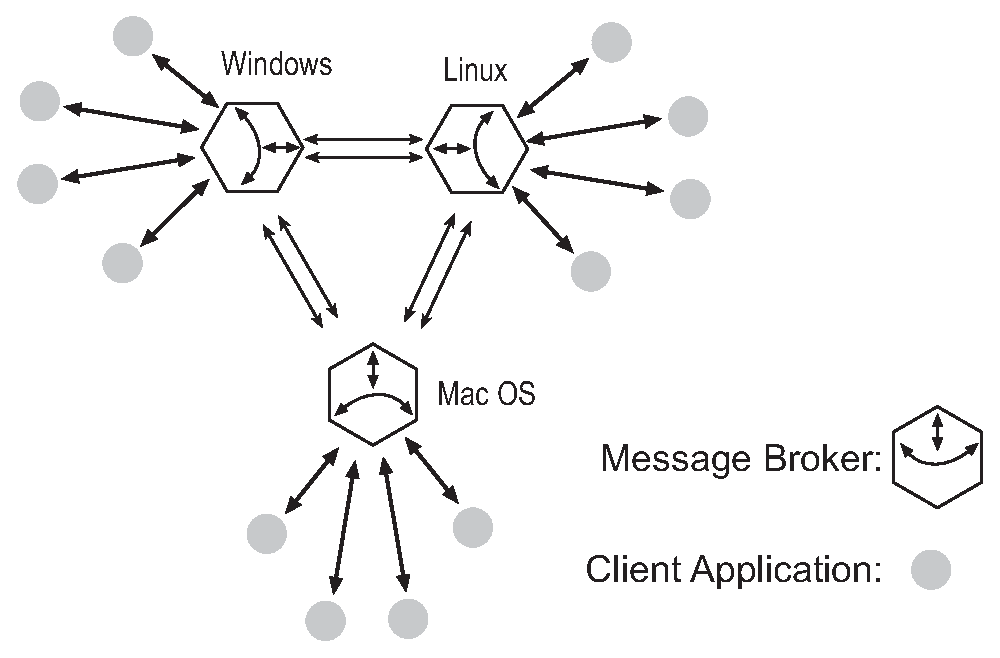
\includegraphics[width=4.6in,height=2.7in]{sbwFig.eps}
\end{center}
\caption{The Systems Biology Workbench (SBW) is a dynamic open-source 
distributed system. Client modules can attach and detach at runtime. 
Client modules can be written in a variety of languages,
including, C/C++, Java, Delphi, FORTRAN, Python, Perl, Matlab, any .NET language.
Data is exchanged between modules via binary messages which can include any combination
of bytes, integers, floating point, complex numbers, strings, arrays and lists. Currently the available modules include, simulators, model editors, SBML manipulation, math library, frequency analyzer, bifurcation discover and analysis modules, structural analysis modules and others. Further details to be found at \url{www.sys-bio.org}}
\end{figure}

An SBW module (the client) provides one or more interfaces or services. Each
service provides one or more methods. Modules register the
services they provide with the SBW Broker. The module optionally
places each service it provides into a category. By convention, a
category is a group of services from one or more modules that have
a common set of methods.

One of the key advantages of SBW is it's language and OS
neutrality. At a stroke this eliminates the irrational language and operating
systems 'wars' that often plague software development. In addition
to providing support for multiple languages there is also the facility to
automatically generate web services from any SBW module (Frank Bergmann, personal communication).

\subsubsection*{Messaging Protocols}

At the heart of SBW is the messaging protocol used to exchange
information between the different modules. For efficiency reasons,
messages that are exchanged between modules are simple sequences
of binary data. For each programming language there is a language
binding library which takes care of much, if not all, of the
housekeeping necessary to operate through SBW, including
connection and transmission of data. In addition, issues such as
little and big-endian byte ordering need not concern the developer
as this is taken care of automatically by the binding libraries.
Each binding also provides the necessary message packing and
unpacking logic and exposes functionality in the form of an
easy-to-use API.

Since SBW message passing is based on TCP/IP sockets it is straight forward
to run SBW across the internet or more significantly across computational nodes
on a supercomputer cluster.

\subsection{BioSPICE}

BioSPICE (\url{www.biospice.org}) is a DARPA funded effort to
develop an open source framework and tool-set for modelling
dynamic cellular network functions. The central component of
BioSPICE is the dashboard which is used to construct work-flows
between BioSPICE enabled applications. Both SBW and the dashboard
encourage code reuse although in different ways. In the dashboard,
code reuse is through the construction of work flows, in SBW code
reuse is via programmatic interfaces and a plugable runtime
architecture. The unit components in SBW tends to be more fine
grained compared to BioSPICE modules. For example, SBW provides
modules such as SBML support, frequency analysis, simulation
methods, bifurcation analysis, which can be tied together at runtime to give the
impression of a single application. The BioSPICE dashboard on the
other hand allows the user to construct fixed work-flows prior
to a run. The workflow configurations cannot be changed during runtime. In addition, where as SBW connects modules via interface specifications, the dashboard connects modules via data types. The BioSPICE dashboard is based on the Java netbeans application which makes it highly Java centric and interaction with applications written in other
languages, though not impossible, non-trivial. It is possible to easily connect
SBW modules to the dashboard (via the SBW Java interface) which greatly increases the
flexibility of the dashboard combining the advantages of a
work-flow approach to the free-flow approach of SBW.

\subsection{BioUML}

BioUML (\url{www.biouml.org}), developed by Fedor Kolpakov
and his team, is a Java framework based around eclipse and targeted
at the systems biology community. The authors state that the
utility of BioUML covers access to databases with experimental
data, tools for formalized description of biological systems
structure and functioning, as well as tools for their
visualization and simulations. BioUML is at an early stage of
development but the central idea is of a plugable environment
where plugins written in Java are used to extend the functionality
of the framework.  Much work remains to make the BioUML usable for
the average biologists but the idea is interesting although the
requirement to write all code in Java is limiting and some means
to permit alternative language bindings would be useful. Recently
the BioUML team developed a SBW interface, which permits
access to plugins that are written in many different languages.

\section{Applications}

In recent years there has been a proliferation of software applications for the systems biology community (See Figure \ref{Apps:Graph}).

\begin{figure}[h]
\begin{center}
  \includegraphics[width=4in,height=2.2in]{ToolsPerYear.eps}
\end{center}
\caption{The Release of Software Tools for Computational Systems Biology over Time. Note the spike in the last five years}
\label{Apps:Graph}
\end{figure}

On the whole, many of these applications provide very similar functionality. The distinguishing feature among them is how easy they are to install and use. The more mature applications tend to be easier to install and have a much richer repertoire of functionality. Many of the applications are simple wrappers around standard ODE or Gillespie solvers and provide a simple means to load models and run time courses. Some of the applications fall by the wayside because the author has lost interest or funding has stopped. It is important therefore that what ever tool one uses, that the ability to export and import a recognized standard (or at least a documented format) such as SBML and/or CellML be available.

The original intention in this section was to list as many of the applications as
possible together with their capabilities but given the large
number now available it soon became clear that this task would be
too great. Instead I refer the reader to the recent paper by Hucka
et. al.\ (2004) where the authors describe almost forty
applications. An even larger list can be found at the sbml.org web
site.

There are some applications however that are worth mentioning specifically because they have some special characteristic. Table 1 lists a number of applications which are being actively maintained, have a reasonably large user base and offer facilities that are either unique or well done. I have not mentioned any stochastic simulators in Table 1 because
many of these are still immature.

\medskip
\begin{table}
\label{table:Apps}
\begin{tabular}{ll}
\rowcolor[gray]{0.8}\color{black}
Application & Description \\ \\
VCell  & A very mature server based application that is specialized \\
       & to build and simulate large scale spatial (PDE) models \\
       & - Open Source, multiplatform \cite{VCELL}. \\
       & \\
Gepasi & This is a forms based application which has been maintained \\
       & for many years by a dedicated author, the tool is \\
       & particularly adapt at carrying out optimizations of ODE \\
       & based models to data - Closed source, Windows, Linux \\
       & \cite{Gepasi:1993}. \\
       & \\
WinSCAMP & A script based GUI application, which like Gepasi has a \\
     & long tradition. Specialized for time course, steady state and \\
     & metabolic control analysis of ODE based models. \\
     & - Source available upon request, multiplatform \\
     & \cite{SauroF91,SauroScamp93} \\
     & \\
Pysces & This is a very complete ODE based simulation environment \\
       & built around the scripting language Python \\
       & - Open Source, multiplatform \cite{Pysces2005}. \\
       & \\
Jarnac/JDesigner & Jarnac is a script based application, JDesigner \\
      & (See Figure 3) is a visual design tool which can use Jarnac \\
      & via SBW to carry out simulations. The simulation capabilities \\
      & of Jarnac are quite extensive, offering both ODE and stochastic \\
      & simulation - Open Source, Windows, Linux \\
      & \cite{sauro:2000,Sauro:Omics}. \\
      & \\
\hline
\end{tabular}
\caption{Mature and Easily Accessible Tools for Modelling Cellular Networks.}
\end{table}

% jigCell?
% bioTapestry?

\medskip
There are also more general purpose tools available, both commercial and open-source which are worth considering. Probably the most well known commercial tool is Matlab (\url{www.mathworks.com}). Although Matlab is an excellent prototyping tool if suffers from poor performance when simulating systems larger than about thirty species if the model is not specified in the correct way. In fact a number of the open-source tools are orders of magnitude faster than Matlab. This stems from the fact that Matlab is a general purpose tool whereas the open-source tools are specialists and are therefore more heavily optimized for their specific application. The commercial tools require a high degree of programming skill because they do not have facilities for representing models in a way familiar to most biologists, instead users are required to derive the differential equations explicitly. Platforms, such as SBW make available translators from SBML to a variety of formats including Matlab, and in a number of cases, users employ tools such as JDesigner to maintain the model, but use a translator to generate Matlab (or any other supported format such as C or Java).

In addition to generic commercial modelling tools there are also now available a number
of commercial tools specifically geared for modelling cellular networks. The most well known
include Gene Networks Sciences, Berkeley Madonna and Teranode (These can easily be located on the web by using a reliable search engine).

\subsection{Model Analysis}

As a user, one of the most important aspects that I consider is the range of techniques that
are available for analyzing the model. The purpose of building a model is not simply to generate
a predictive tool, if it were we could probably get away with using empirical statistical techniques or machine learning approaches such a neural nets. An additional important role of model building is also to gain a deeper understanding into the properties of the model and to understand how the structure of the model leads it to behave the way it does. In order to answer these kinds of questions one needs techniques that can interrogate the model in a variety of different ways.

Table 2 lists some of the most important techniques that are available for analyzing models. Without these techniques, a model will often be as difficult to understand as the real system it attempts to model; the application of these techniques is therefore important.

\begin{table}[h]
\label{table:techniques}
\begin{tabular}{ll}
\rowcolor[gray]{0.8}\color{black}
Approach & Description \\ \\
Connectionist Theory & Connectivity studies are centered around the search for \\
                     & patterns in the way cellular networks are physically \\
                     & connected. \cite{BarabasiReview2004} \\
                     &  \\
Structural Analysis & There are a wide range of useful techniques which focus \\
                    & on the properties of the networks that depend on the \\
                    & mass conservation properties of networks. These \\
                    & include, conservation analysis, flux balance and \\
                    & elementary mode analysis \cite{Schuster:Book}. \\
                    & \\
Cellular Control Analysis & CCA (also known as metabolic control analysis) \\
                    & is a powerful technique for analyzing the \\
                    & propagation of perturbations through a network. \\
                    & There exists a very large literature describing \\
                    & applications and theory \cite{Fell:Book}. \\
                    & \\
Frequency Analysis  & Closely related to CCA is the analysis of how signals \\
                    & propagate through a network \\
                    & \cite{Ingalls2004,RaoSauroArkin}. \\
                    & \\
Bifurcation Analysis & Bifurcation analysis is concerned with the study \\
                     & of how the qualitative behavior of steady state \\
                     & solutions change with changes in the \\
                     & model parameters \cite{TysonNatReview2001}. \\
\\ \hline
\end{tabular}
\caption{Model Analysis Methods}
\end{table}

All these techniques are extremely useful in gaining insight into how a model operates. The connectionist and structural analyses focus on the network properties of the model, that is they
do not explicitly consider the dynamics of the model but on how the network connectivity sets the stage for generating the dynamics of the model. The last three techniques, CCA, frequency analysis and bifurcation analysis focus on the dynamical aspects of a model and are crucial to
gaining a deep insight into the model \cite{Bakker:1997,TysonNatReview2001}.

\subsection{Model Fitting and Validation}

An important activity in systems biology modelling is the need to fit experimental data
to models. There isn't sufficient space to cover to any great detail this topic but as
time series data from microarray, proteomic and metabolomic data becomes more readily available
the need to fit models to experimental data will become more acute. There are a number of issues
related to this topic, one concerns the nature of the data that is generated by most of the current experimental techniques. In particular, most current techniques generate normalized data, that is absolute values are not given. This poses a number of problems to a fitting
algorithm, since the underlying model is in terms of absolute quantities. A number of solutions
are potentially available, however none are entirely satisfactory and ultimately the models generated by normalized data will most likely be only capable of reproducing trends in the
data. Whether such models will have great predictive value is open to question and much research remains to be done in this area.

The other issue, is the intensive nature of the computations that are required to fit even a moderately sized model. One of the necessary requirements for fitting a model is estimating the confidence limits on the fitted parameters and the range of parameter space which describes the experimental data. This information is crucial to determine
the validity of the model and can be used to design additional experiments to either refute the model or increase the precision of the model parameters. As a result of these requirements, computing a global optimization can take a considerable time. For example, in a recent study, Vijay Chickarmane (unpublished) estimated that the time required to fit a model of approximately three hundred parameters would be of the order of seven years on a normal desktop computer. Luckily, global optimization can be easily parallelized given a suitable optimizer (for example a genetic algorithm based optimizer) and the computation time can be reduced by hosting the problem on a cluster machine. Chickarmane estimates that using a one thousand node cluster, the optimization of a three hundred parameter model can be reduced to approximately two days of computation time. Such a computation can be easily setup using SBW. A single node on the cluster would act as the primary optimizer; this node in turn would farms out the time consuming simulation computations to the remaining nodes on the computer. For very large models, Grid computing \cite{GridComputing:Abbas} may be very appropriate for solving this kind of problem.

\section{Future Prospects and Conclusion}

The Systems Biology field has been developing rapidly in recent years but much remains to be done. One of the most useful developments must undoubtedly go to the development of standards such as SBML and CellML. Indeed the most recent of a long list of new systems biology journals, (Molecular Systems Biology) has stipulated that SBML is the preferred format for contributing models, hopefully other journals will follow. However, one aspect that still remains to be dealt with is to formalize the sematic rules for SBML. At the moment there is no guarantee that models written by different tools can be interchanged. If one focuses on the core specification in SBML that this is generally not an issue but it is vital that sematic validators be developed for SBML.

The other area that has received a lot of attention in recent years is the development of tools for systems biology. However, much of what is being developed is repetitious and little true advancement is being made. This is probably do to the large number of new comers to the field who are inexperienced and inevitably repeat what has gone before. A number of solutions exist to solve this problem, one is to develop extensible frameworks such as SBW, BioSPICE or BioUML, the other is to develop a suite of open-source libraries which can carry out specific functionality. An example of this is libSBML being developed by the SBML team. This library, written in C/C++ for maximum portability, enables other developers to concentrate on simulation capability rather than waste unnecessary effort developing their own SBML parser.  In terms of other possible libraries, examples include, open-source Gillespie based stochastic solvers and ODE solvers. In both cases there is also the need to develop scalable and robust methods for computing the dependent and independent species. Further more, hybrid methods combining continuous and stochastic methods is a pressing need at the current time. Many biological systems interface noisy sensory apparatus (e.g. ligand binding to the surface of a cell membrane) to internal continuous analog networks \cite{SauroReview:2004}. In addition to the core solvers, we also need scalable analysis tools, particularly bifurcation analysis tools and sensitivity analysis tools. On the model validation front, much remains to be done, particularly the relationship between model validation and how this can direct future experimentation. This leads on to the development of new methods and algorithms for analyzing the complex networks in particular methods should be developed to modularize large networks since understanding an entire network is virtually impossible with out some recourse to a hierarchical modularization.

Finally, the role of high performance computing in systems biology is still very novel. In fact there appear to be very few applications to date of high performance computing to systems biology. One of the few useful applications is model fitting to data. When done correctly, this is an extremely computationally intensive calculation and is an ideal candidate for large cluster machines. In fact, one wonders whether this is the application for systems biology which could benefit from Grid computing.

\section{Recommended Resources}

Four web sources which are of interest to readers of this chapter include:

\url{\bf http://www.cellml.org} This is the main CellML site. It has a very
rich set of models expressed in CellML including specifications for the
standard and pointers to software toolkits.

\url{\bf http://www.sbml.org} This is the main SBML site. The site as ample documentation,
examples illustrating how SBML is and should be used. In addition is has a rich set of software
tools, in particular libSBML, which allows developers to easily add SBML support to
their tools.

\url{\bf http://www.sys-bio.org} This is the main SBW (Systems Biology Workbench) site. The latest versions for SBW, developer documentation, example models, screen shots, user guides can be obtained from this site. A link to the main sourceforge site is given where all the source code for SBW is made available.

\url{\bf http://www.biospice.org} This is the main BioSPICE site. This site includes
a description of BioSPICE and the large number of tools now available for the BioSPICE
dashboard (including SBW itself).

\section{Acknowledgements}

I would first like to acknowledge the generous support from the Japan Science and Technology Agency, DARPA (BAA01-26 Bio-Computation) and the US Department of Energy GTL program, without  which the bulk of the work described in this chapter would not have been carried out. I would also like to acknowledge Mike Hucka, Andrew Finney and Hamid Bolouri for their initial work on the Systems Biology Workbench and in more recent years the tremendous programming work done by Frank Bergmann and the critical support given by Sri Paladugu and Vijay Chickarmane to the development of novel computational methods in Systems Biology.


\bibliography{mybib}
\bibliographystyle{ajhg}

\end{document}

